\lab{Algorithm}{The Knapsack Problem}{The Knapsack Problem}
\label{lab:Knapsack}

\objective{This section teaches about NP-hard problems, particularly the knapsack problem.}

\section*{The Knapsack Problem}

\begin{figure}
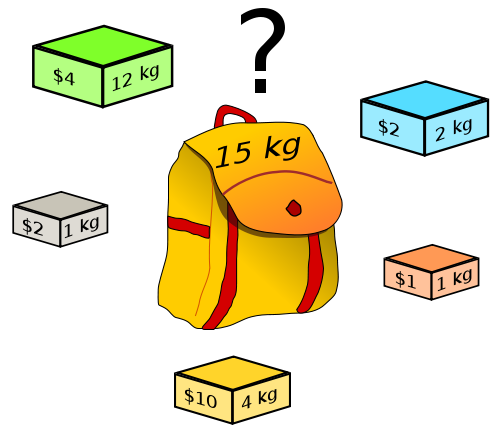
\includegraphics[width=\textwidth]{Knapsack.png}
\caption{Visualization of the Knapsack problem TODO: Make a picture similar to this}
\end{figure}

You are given a knapsack that can only hold a certain weight.
You have a plethora of items that have value and weight.
You want to find the combination of items that have the most value with out exceeding the weight.
This is the 2 dimensional knapsack problem.
Will focus on the 0/1 knapsack problem, which states that each item must be put in entirely or not at all.

A three dimensional version the items would have volume and the knapsack can only hold an certain volume as well as weight. 

This problem is has many different applications for decision making in a wide variety of fields.
Two examples are finding the least wasteful way to cut raw materials and the selection of capital investments in financial portfolios.
This problem often appears in problems involving resource allocation and financial constraints.

\begin{problem}
Write a function that solves the Knapsack problem by testing all possible combinations of items and choosing the combination with the most value that meets the weight constraint.
Only test it up to 15 objects.
\end{problem}

This way finds the optimal solution, but there is a problem.
Given $n$ objects the number of combinations is $2^n$.
The complexity of the problem grows very quickly.
For example: if you had 50 items, it would take more than 10 years to compute the optimal solution.
For all the following timing problems let your items have values between 1 and 100 and weights between 1 and $\frac{Capacity}{10}$.

\begin{problem}
Time the Knapsack problem for $11-20$ items with a carrying capacity of $10,000$.
Plot the times.
What is the complexity of the algorithm for increasing the number of items?

\begin{figure}[H]
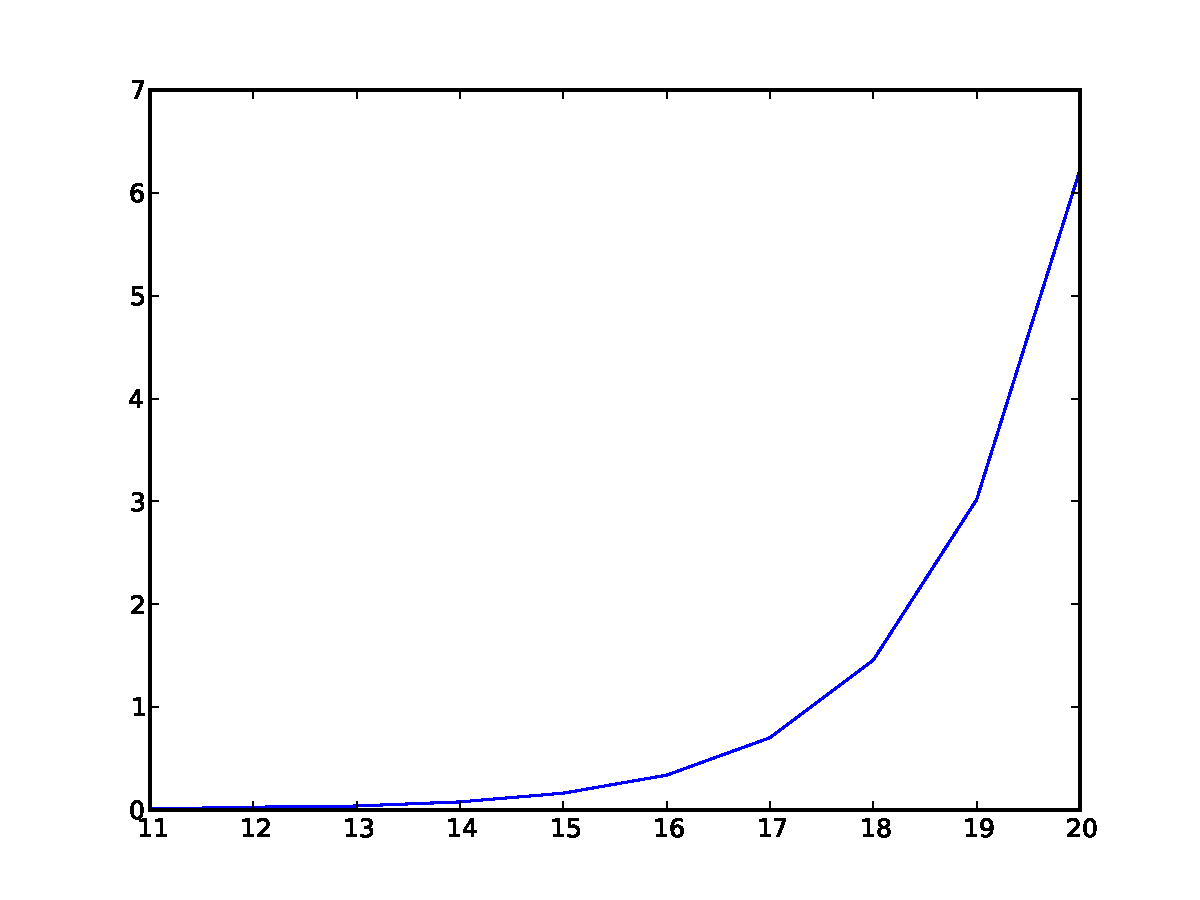
\includegraphics[width=\textwidth]{naiveTime.pdf}
\caption{
Your graph should look similar to this.
As you can see as the number of items increases time increases exponentially}
\end{figure}
\end{problem}

\begin{problem}
Time that algorithm for the carrying capacities $10,000-90,000$ every multiple of $10,000$ with $15$ items.
Plot the times.
What is the complexity of the algorithm for increasing the weight?

\begin{figure}[H]
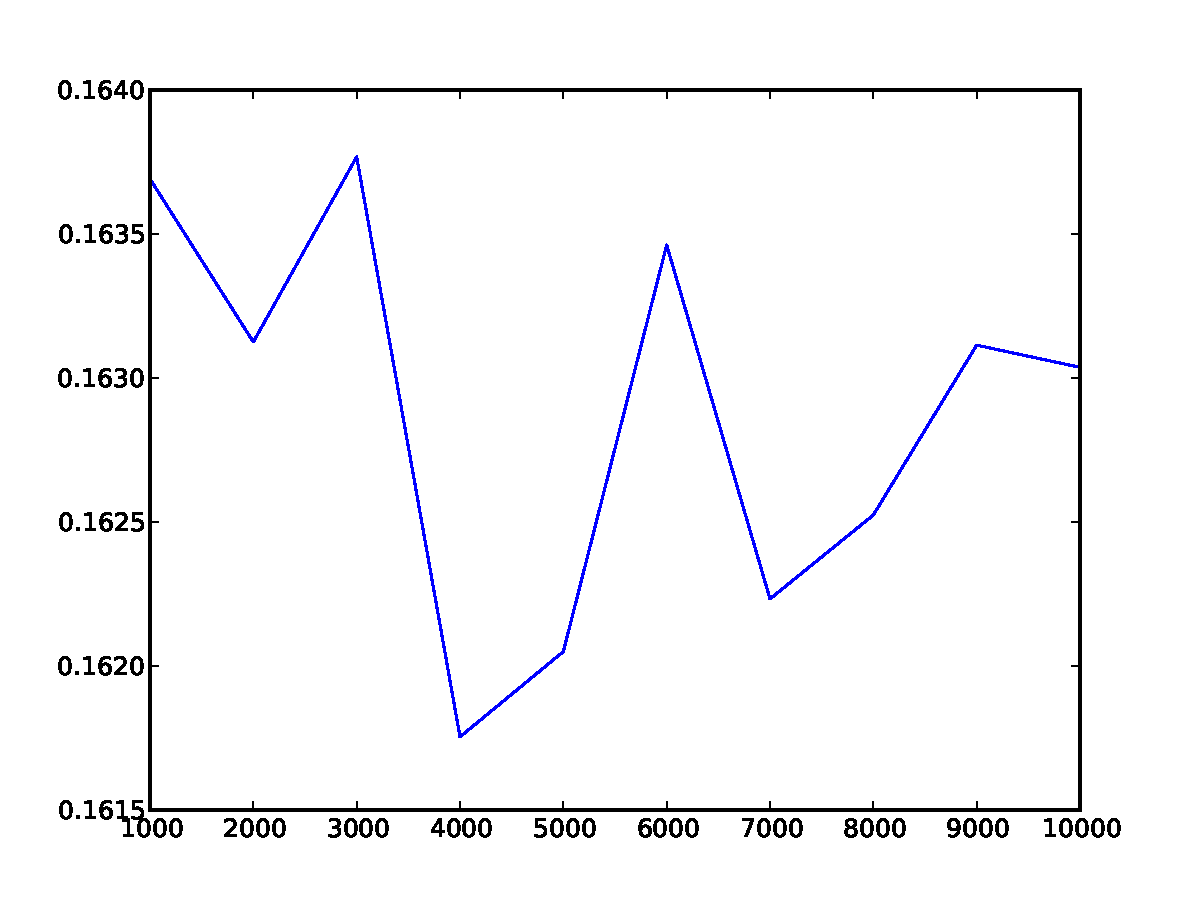
\includegraphics[width=\textwidth]{naiveWeight.pdf}
\caption{
Your graph should look like this.
The weight of the items has essentially no effect on the time.}
\end{figure}
\end{problem}

\section*{NP-Hard}

Any problem that is not polynomial time is known as NP-hard.
The Knapsack Problem is an NP-hard problem since it is $\mathcal{O}\left(2^n\right)$ where $n$ is the number of items that are available.
Using the branch and bound approach we can find the optimal solution in psuedo-polynomial time.

\section*{Branch and Bound method}

We calculate the optimal solution using only the first $i$ items for weights 0 through W (where W is the maximum weight the knapsack can hold).

(ALGORITHM DESCRIPTION NEEDS REVISION)
We do this by initializing the 0th row to be empty.
For the $i$'th row (where $i>0$) we go through $j$ from 1 through W.
If the ith element's weight is more than j then the optimal combination is the same as it was for i-1.
If ith element's weight is less than j, then we compare the combination at i-1 at weight j to the combination i-1 at the weight j-the ith element weight plus the ith element.
Whichever one has a higher value is the optimal combination using the first ith elements less than or equal to the weight of j.
You continue this until you have done all n elements.
The combination using n items with a weight of W is guaranteed to be the optimal combination.

This only does $W*n$ checks, so it is a lot faster.
This works by eliminating combinations that could not be the optimal solution.

\begin{problem}
Write a function that solves the Knapsack problem using the branch and bound method.
\end{problem}

\begin{problem}
Time the Knapsack problem for $11-20$ items with a carrying capacity of $10,000$.
Plot the times.
What is the complexity of the algorithm with respect to the number of items?
For the items, use the specifications given for the previous timing problems.

\begin{figure}[H]
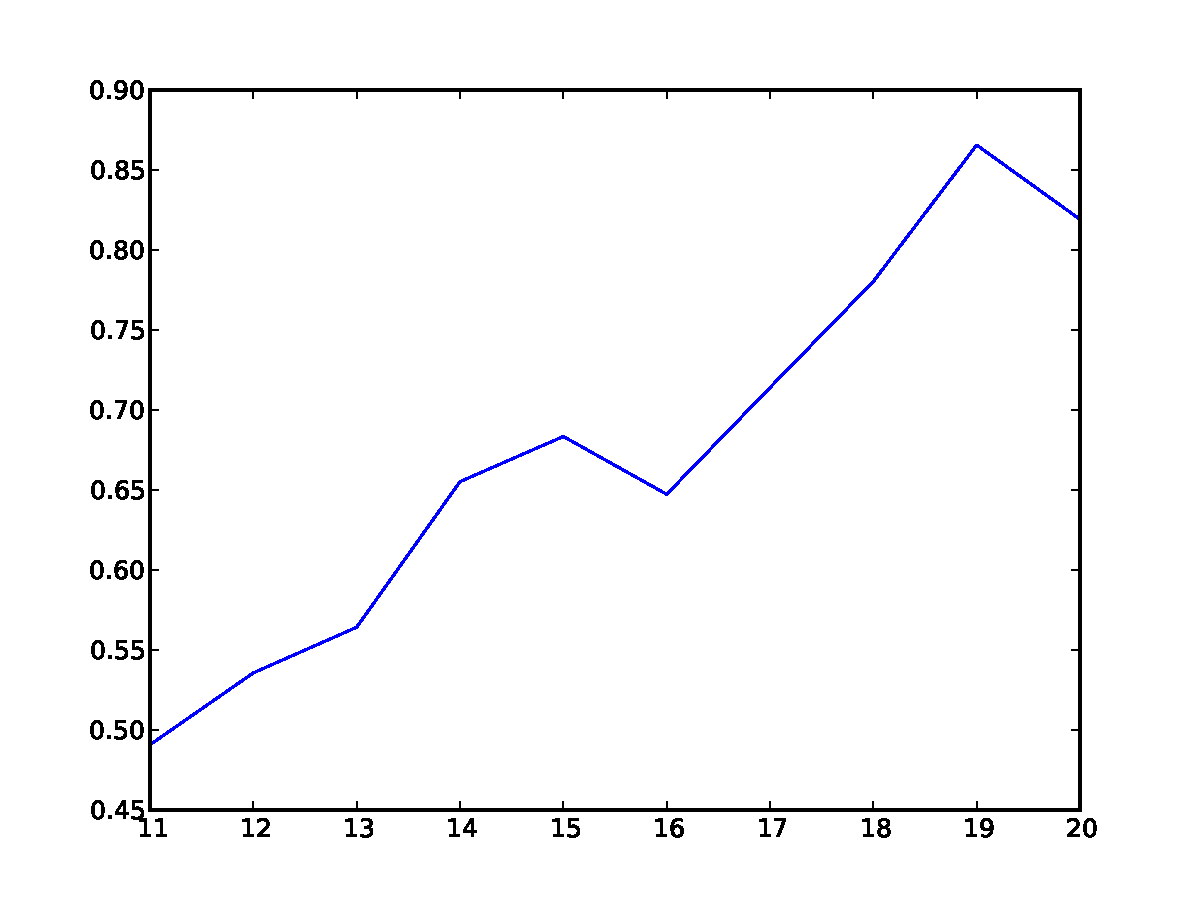
\includegraphics[width=\textwidth]{dynamicTime.pdf}
\caption{
Your graph should look similar to this.
As the number of items increases time increases linearly}
\end{figure}
\end{problem}

\begin{problem}
Time the branch and bound algorithm for the carrying capacities $10,000-90,000$ every multiple of $10,000$ with $15$ items.
Plot the times.
What is the complexity of the algorithm with respect to weight?

\begin{figure}[H]
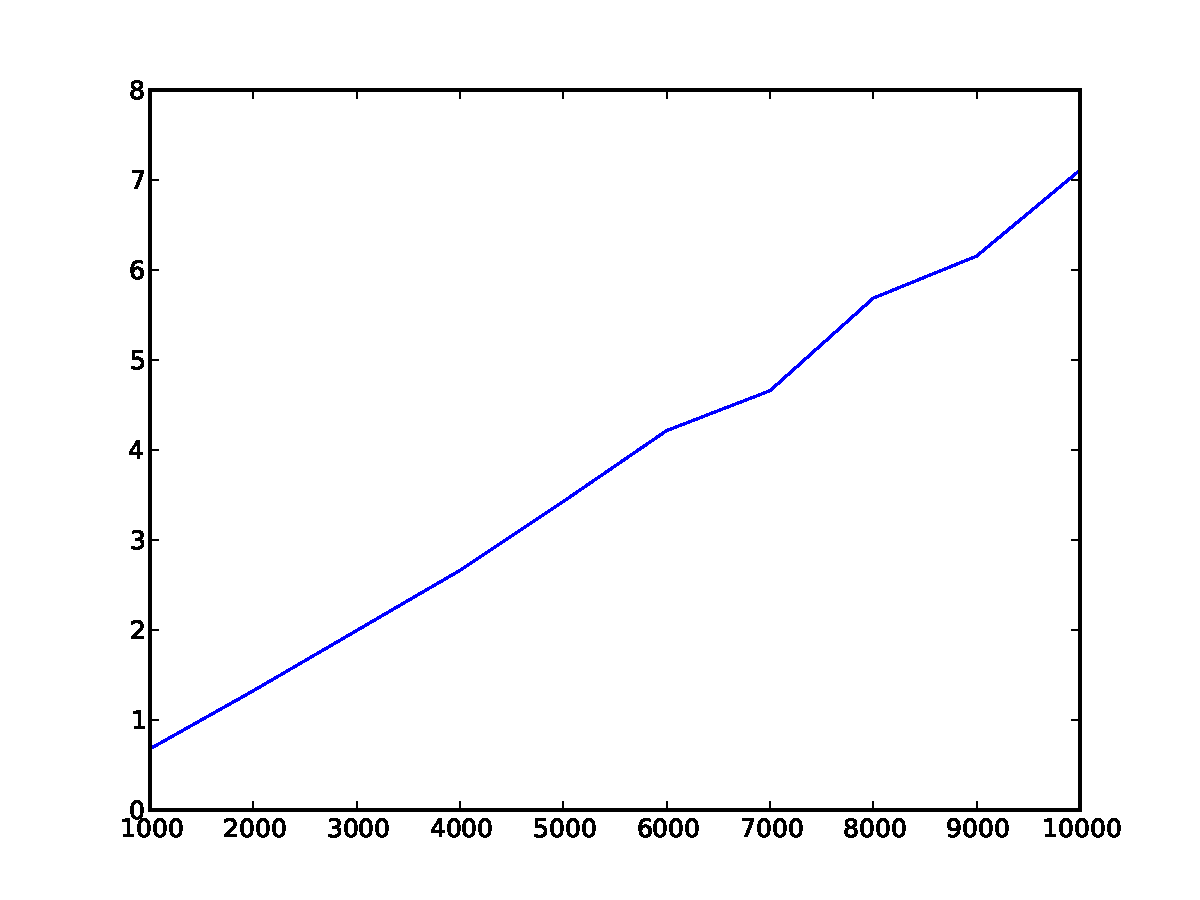
\includegraphics[width=\textwidth]{dynamicWeight.pdf}
\caption{
Your graph should look similar to this.
As the weight of items increases time increases linearly}
\end{figure}
\end{problem}